\begin{center}
\begin{figure}[H]
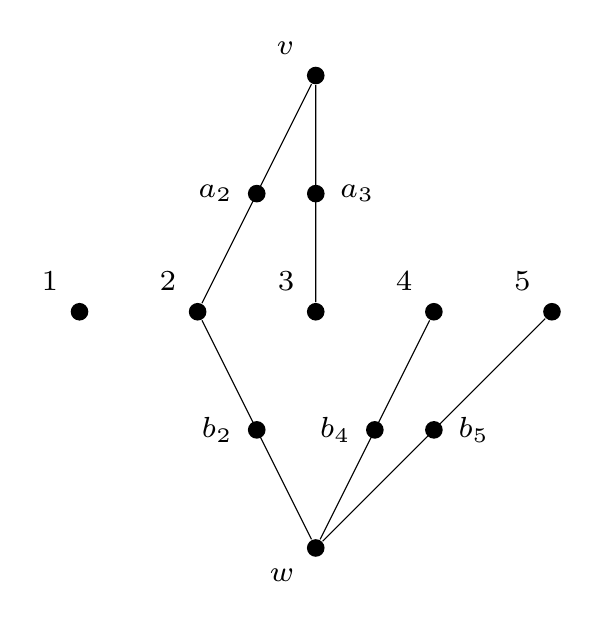
\begin{tikzpicture}[scale=1.5, transform shape]

\node[circle, label=above left:{\scriptsize 1}, fill=black, inner sep=1.5pt] (1) at (1,0) {};
\node[circle, label=above left:{\scriptsize 2}, fill=black, inner sep=1.5pt] (2) at (2,0) {};
\node[circle, label=above left:{\scriptsize 3}, fill=black, inner sep=1.5pt] (3) at (3,0) {};
\node[circle, label=above left:{\scriptsize 4}, fill=black, inner sep=1.5pt] (4) at (4,0) {};
\node[circle, label=above left:{\scriptsize 5}, fill=black, inner sep=1.5pt] (5) at (5,0) {};

\node[circle, label=above left:{\scriptsize $v$}, fill=black, inner sep=1.5pt] (v) at (3,2) {};
\node[circle, label=below left:{\scriptsize $w$}, fill=black, inner sep=1.5pt] (w) at (3,-2) {};

\draw (v) -- (2) node[midway, circle, fill=black, inner sep=1.5pt, label=left:{\scriptsize $a_2$}] {};
\draw (v) -- (3) node[midway, circle, fill=black, inner sep=1.5pt, label=right:{\scriptsize $a_3$}] {};

\draw (w) -- (2) node[midway, circle, fill=black, inner sep=1.5pt, label=left:{\scriptsize $b_2$}] {};
\draw (w) -- (4) node[midway, circle, fill=black, inner sep=1.5pt, label=left:{\scriptsize $b_4$}] {};
\draw (w) -- (5) node[midway, circle, fill=black, inner sep=1.5pt, label=right:{\scriptsize $b_5$}] {};

\end{tikzpicture}
\caption{A $\DISJ$ embedding into $\CTRAV$ with $n = 5$. There is a path from $v$ to $w$ if and only if $\exists i \in [n]$ with $x_i = y_i = 1$.}
\label{fig:ctrav-gadget}
\end{figure}
\end{center}